\section{Empirical Evaluation}


\begin{figure*}[th]
\centering
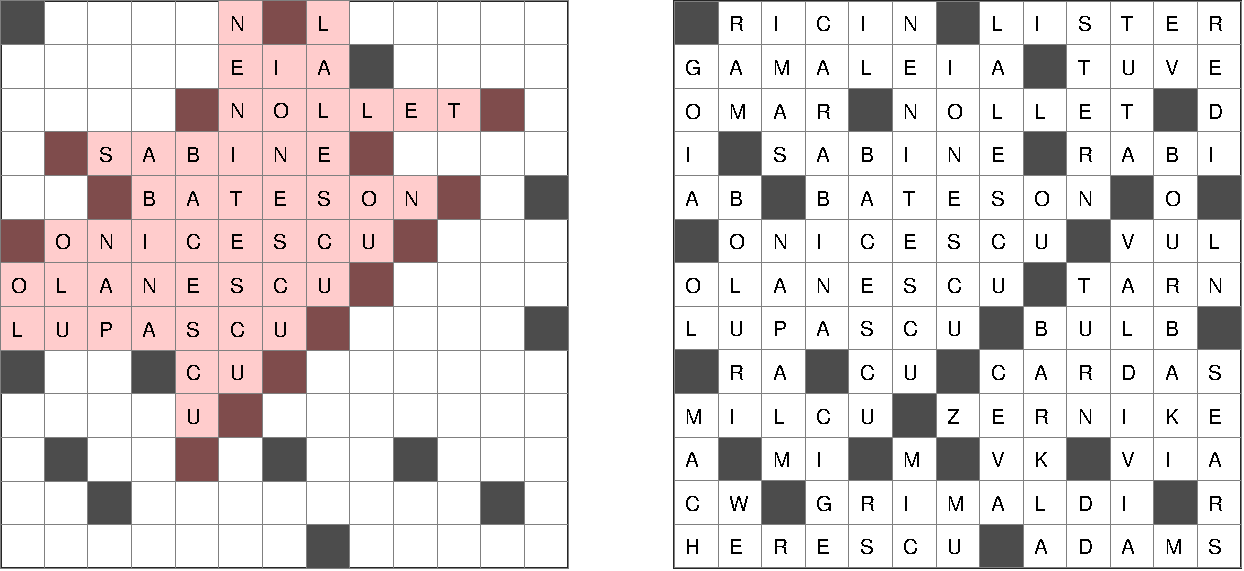
\includegraphics[width=0.56\textwidth]{_empiricalSupport/y-2013/results/_runWombat/mrmeGrids_y2013-60x932-14400x352-14113466-paper.pdf}

\vspace{0.15cm}

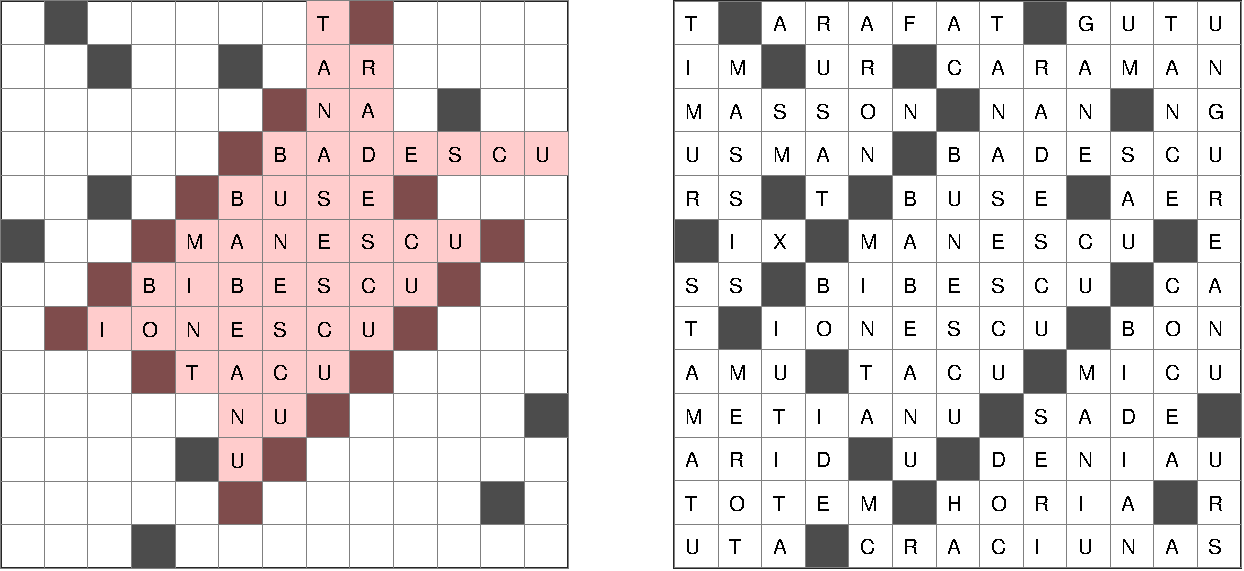
\includegraphics[width=0.56\textwidth]{_empiricalSupport/y-2021/results/_runWombat/mrmeGrids_feb3-60x38035-14400x224-13741779-paper.pdf}

\vspace{0.15cm}

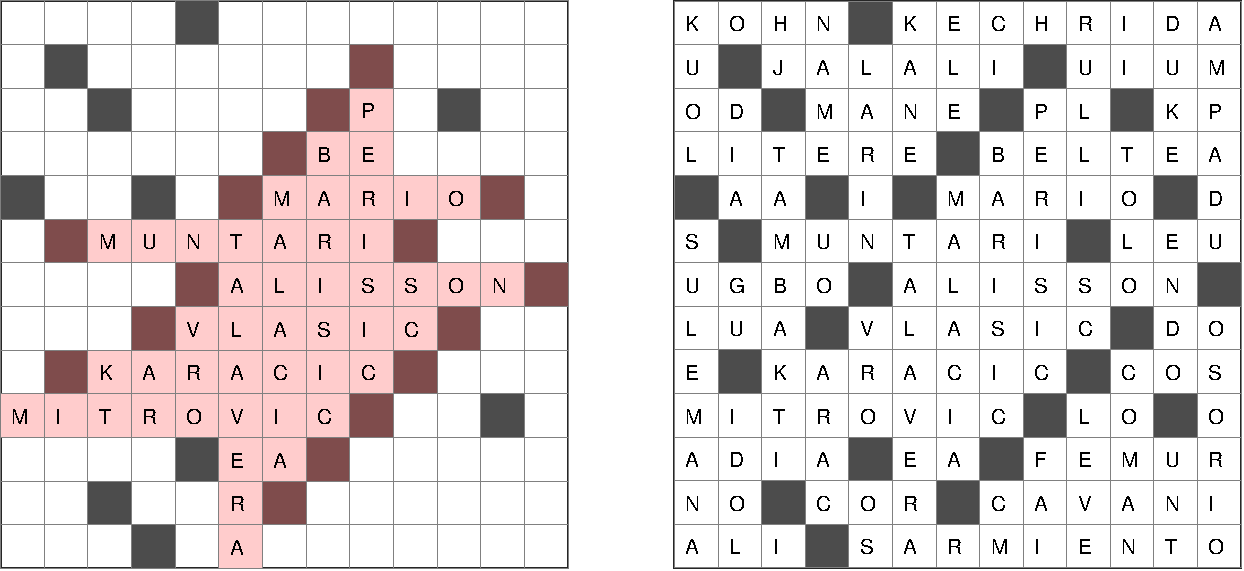
\includegraphics[width=0.56\textwidth]{_empiricalSupport/y-2023/results/_runWombat/mrmeGrids_y2023-60x446-14400x352-14179462-paper.pdf}

\caption{Top results for years 2013 (top row), 2021 (middle) and 2023 (bottom). Left: seeds after
placing additional black cells. Right: {\sc Wombat} solutions,.}
\label{fig:results}
\end{figure*}

We applied the approach presented above to synthesize grids for three years of the competition: 2013, 2021 and 2023. Each year uses its own thematic dictionary. Note that competition results and human-designed grids for year 2023 are not yet announced.

For each of the three years we generated and expanded cores (lines~\ref{algl:generateCores} and \ref{algl:expandCores} in Algorithm~\ref{algo:core-exp}), generated seeds (line~\ref{algl:generateSeeds}) that were then ranked (line~\ref{algl:rankSeeds}). Top-ranked seeds were then evolved (line~\ref{algl:evolveSeeds}). The number of seeds ranked and top-ranked seeds evolved are listed in Table~\ref{tab:rankingEvolving}.


The ranking and evolution steps were repeated four times for the same seed set for each year. Each run used a different random-number generator initialization. As per Section~\ref{sec:evolution}, each ranking + evolution run took about two days on a $32$-core CPU. We used four $32$-core CPU nodes on a grid and thus were able to execute all four runs in parallel. The highest score grids synthesized for each year are shown in Figure~\ref{fig:results}. At the left, we show evolved seeds, with the contents of the original seed
shown in tinted background, and new black cells added during the evolution as solid black cells.

The human competition publishes the top 12 entries every year.
Years 2013 and 2021 feature in their top-12 entries at least one entry that contains the $6 \times 4$ pattern
considered in our experiments (Figure \ref{fig:pattern} left).
In 2013, scores in the top 12 list ranged from 184 (first place), to 181 (second place), and so on down to 175 on the twelfth place.
Our score for that year is 182.
In 2021, human scores in the top-12 list range from 195 down to 187, whereas our score is 190.
Two top-12 entries in 2021 feature the perfect-score pattern considered in our work.
One has 194 points, and one has 189 points. Our entry has 190 points, and it turns out to be similar to the 194 entry. 
2023 human results are not announced yet. We report a score of 186.

Thus, with additional input as simple as a pattern to use, which 
in our experiments
is a $6 \times 4$ rectangle with two black cells in two corners,
our approach can reach scores that are competitive with top human performers.
Part of the previous work utilized much more detailed additional input, such as the entire configuration of black cells~\cite{DBLP:conf/socs/BoteaB21}.
Other previous work did not utilize such input, but the performance lagged significantly behind
top results~\cite{DBLP:conf/cig/BulitkoB21}.


%\vb{Adi: please comment on how good those results are and where this places us among the competition grids for those years.}

%\vb{Adi: please also remind the reader how little initial information the process needed to derive those grids (so that the reader does not think we took published human grids and did something to them}

